\documentclass[11pt,a4paper]{article}
\usepackage[hmargin=23mm,vmargin=17mm]{geometry}
\usepackage{amsmath,amssymb,booktabs,graphicx,hyperref}
\hypersetup{colorlinks=true,urlcolor=blue,linkcolor=black}
\setlength{\parindent}{0pt}
\setlength{\parskip}{.32em}
\title{Reproducing DiffTraj and evaluating speed and vehicle class}
\author{Experimental progress report}
\date{11 November 2026}
\begin{document}
\maketitle
\section{Problem and related work}
A synthetic trajectory is a sequence of positions ordered by time. When several journeys have the same origin, destination and duration, a generator should reproduce the distribution of their paths and movements. Here the first objective is to reproduce DiffTraj on the settings of Zhu et al.\ \cite{difftraj}. The second objective is to measure the contribution of time-varying speed supervision and vehicle type on a dataset that records both.

Different approaches learn different aspects of this distribution. A variational autoencoder learns a distribution of latent variables and decodes sampled variables into observations \cite{vae}. An adversarial generator learns through a discriminator that distinguishes observed and generated samples \cite{gan}. Diffusion training instead constructs noisy versions of each training example and learns to predict the injected noise \cite{ddpm}. In trajectory synthesis this objective can be applied directly to a sequence of coordinates. DiffTraj conditions the prediction on trip attributes and compares the resulting geographical distributions with perturbation, VAE and adversarial baselines. Its published comparison, released denoiser and Chengdu weights provide a reference for evaluating a small modification.

\section{Original model and reproduction target}
A trip $X$ has two standardized coordinate channels and 200 ordered positions. The request vector $h$ contains the departure-time bin, total distance, duration, original number of samples, mean displacement, mean speed, start cell and end cell. Given noise level $t$, a variance schedule $\beta_t$ and independent standard normal noise $\epsilon$, the training input and loss are
\[
 a_t=\prod_{k=1}^t(1-\beta_k),\qquad
 X_t=\sqrt{a_t}X+\sqrt{1-a_t}\,\epsilon,\qquad
 L_0=\mathbb E\|\epsilon-f_\theta(X_t,t,h)\|^2 .
\]
Here $f_\theta$ is a temporal U-Net. Convolutions at several resolutions describe local and longer segments of motion. The condition encoder combines continuous trip descriptors with embeddings of the departure bin and endpoint cells. At generation time the model starts with Gaussian coordinates and applies successive noise estimates. The release uses 500 noise levels and 100 deterministic DDIM transitions \cite{ddim}.

The paper's Table~1 uses 3,000 generated trips per method in each of two cities. Density compares grid occupancy. Trip compares the joint start and end cells. Length compares distributions of total distance with consecutive positions joined by line segments. These three errors use Jensen--Shannon divergence, the mean divergence of the two distributions from their average, and smaller values indicate closer agreement. Pattern compares frequent spatial cells using the harmonic mean of precision and recall. The published target and the status of independent replication appear below.
\begin{center}\begin{tabular}{lrrrr}\toprule
Published target & Density & Trip & Length & Pattern\\\midrule
Chengdu & .0055 & .0154 & .0169 & .823\\
Xi'an & .0126 & .0165 & .0203 & .764\\\bottomrule
\end{tabular}\end{center}
Replaying the released sampling notebook on a GPU with the Chengdu weights generated 500 trips. After 100 reverse transitions and length restoration, these contained 141,747 finite positions with a median of 259 positions per trip. Figure~\ref{fig:chengdu} shows the resulting paths. Scoring the original two cities requires the observed November 2016 taxi coordinates. The authors confirm that access to these GPS records requires a license. Their Table~5 also gives a public-data benchmark on Porto. The UCI source contains 1,710,670 trip records in the training file. Excluding missing-data flags and retaining at least 120 original points leaves 55,267 complete traces from 439 taxis. The median retained length is 155 positions. These observations support a separate reproduction of the Porto comparison. Independent Table~1 scores remain pending.

\begin{figure}[htbp]\centering
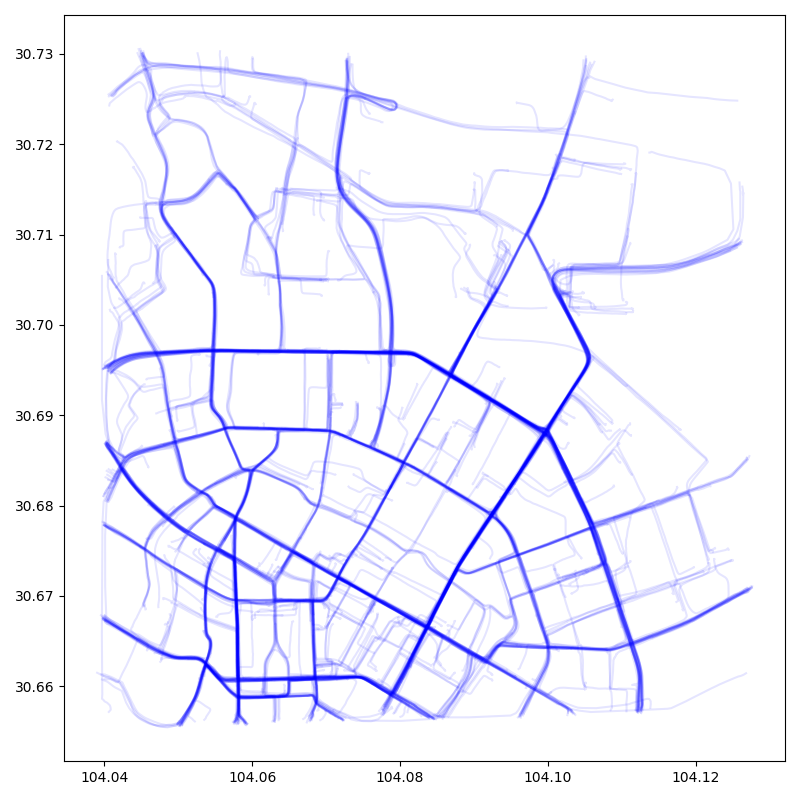
\includegraphics[width=.46\linewidth]{chengdu.png}
\caption{Chengdu trajectories generated from the released weights and example trip descriptors. Each line is one sample. Longitude in degrees is plotted horizontally and latitude vertically. Overlapping samples appear darker.}\label{fig:chengdu}
\end{figure}

\section{Matched experiments on labelled SUMO trajectories}
The supplied simulation table records times, vehicle identifiers, planar positions in metres, scalar speeds in metres per second, and traffic participant labels. We retained vehicle records with a unique class, finite measurements, positive travelled distance, at least 20 observations and gaps of at most two seconds. The resulting corpus contains 136 buses, 173 bicycles, 351 motorcycles, 1,039 private cars and 92 taxis or ride-hailing cars. A deterministic split by vehicle identifier assigns 1,416 vehicles to training and 375 to development. All comparisons use the same 128 development requests with the same trip descriptors and initial sampling noise. Five of these requests are taxis.

The local baseline fits the released coordinate architecture to standardized planar positions sampled at 200 uniformly spaced times per trip. Its original condition vector already includes trip-average speed. For the speed extension, let $\hat X$ be the model's estimate of clean coordinates in metres. For each interval of duration $\Delta t$, its predicted speed is $\hat v_i=\|\hat X_i-\hat X_{i-1}\|_2/\Delta t$. The target $v_i$ is the average observed simulator speed over that interval, obtained by integrating the speed measurements on their original clock. The additional loss is $0.05a_t$ times the mean smooth absolute-error loss (smooth L1) between $\log(1+\hat v_i)$ and $\log(1+v_i)$ with speeds expressed in m/s. Weighting by $a_t$ reduces the influence of unstable clean-position estimates at high noise. Vehicle class enters through a learned embedding added to the conditional trip embedding. Four arms isolate the two changes and their combination.

The local evaluation measures speed from successive coordinates on both reference and generated trips. The speed Wasserstein distance $W_1$ has units of m/s and measures the mean absolute displacement needed to match two one-dimensional distributions. Length $W_1$ uses total trip distances. The local density diagnostic uses a training-bounded $16\times16$ grid, one extra cell for overflow, and natural logarithms. The two training seeds use identical development requests and sampling noise.

\section{Results and decision}
The 2,000-update baseline generated a median interval speed of 128.99 m/s against 11.36 m/s in the simulation reference. Across 100 disjoint pairs of 128 observed development trips, the median speed $W_1$ was 0.41 m/s. A sampler control with known injected noise recovered positions with a root mean squared error of $1.2\times10^{-6}$ m. On 32 observed trips, using the trained network to estimate clean coordinates from noise levels 50, 250 and 495 gave errors of 134 m, 774 m and 58.2 km. We therefore repeated the baseline with 8,000 updates under the same initialization and training and sampling conditions. We then repeated all four 8,000-update fits with a second training seed.
\begin{center}\small\begin{tabular}{rlrrrr}\toprule
Seed & Condition & Speed $W_1$ & Length $W_1$ & Density JS & Outside \\
 & & (m/s) & (km) & & (\%)\\\midrule
42 & Original & 51.64 & 11.38 & 0.119 & 8.2\\
42 & Speed & 14.34 & 1.09 & 0.167 & 14.4\\
42 & Class & 55.74 & 13.35 & 0.146 & 13.0\\
42 & Speed and class & 98.31 & 18.03 & 0.166 & 17.8\\
43 & Original & 9.89 & 0.98 & 0.140 & 6.9\\
43 & Speed & 5.42 & 0.89 & 0.204 & 10.0\\
43 & Class & 32.22 & 4.56 & 0.136 & 6.4\\
43 & Speed and class & 99.66 & 15.24 & 0.160 & 9.2\\
\bottomrule\end{tabular}\end{center}

Extending baseline training lowered speed distribution error from 709.73 to 51.64 m/s and the fraction of generated points outside the training bounds from 88.4\% to 8.2\%. Short trips remained particularly difficult. Across four equally sized groups ordered by duration, speed $W_1$ ranged from 139.55 m/s in the shortest group to 8.94 m/s in the longest. In the shortest group, successive generated points had a median separation of 31.35 m, compared with 4.52 m for observed points.

The table compares two training seeds at 8,000 updates. In each seed, speed supervision alone reduced speed and length error while increasing spatial density divergence. The absolute gain depended strongly on the baseline fit. Class conditioning alone increased speed error in both seeds. The combined model yielded larger motion errors than either baseline. A time-varying target thus improved particular motion statistics under these settings. The class embedding supplied no repeatable improvement on those endpoints. An independent vehicle population is needed to estimate the size of the effect beyond these development requests.

\clearpage\begin{figure}[!ht]\centering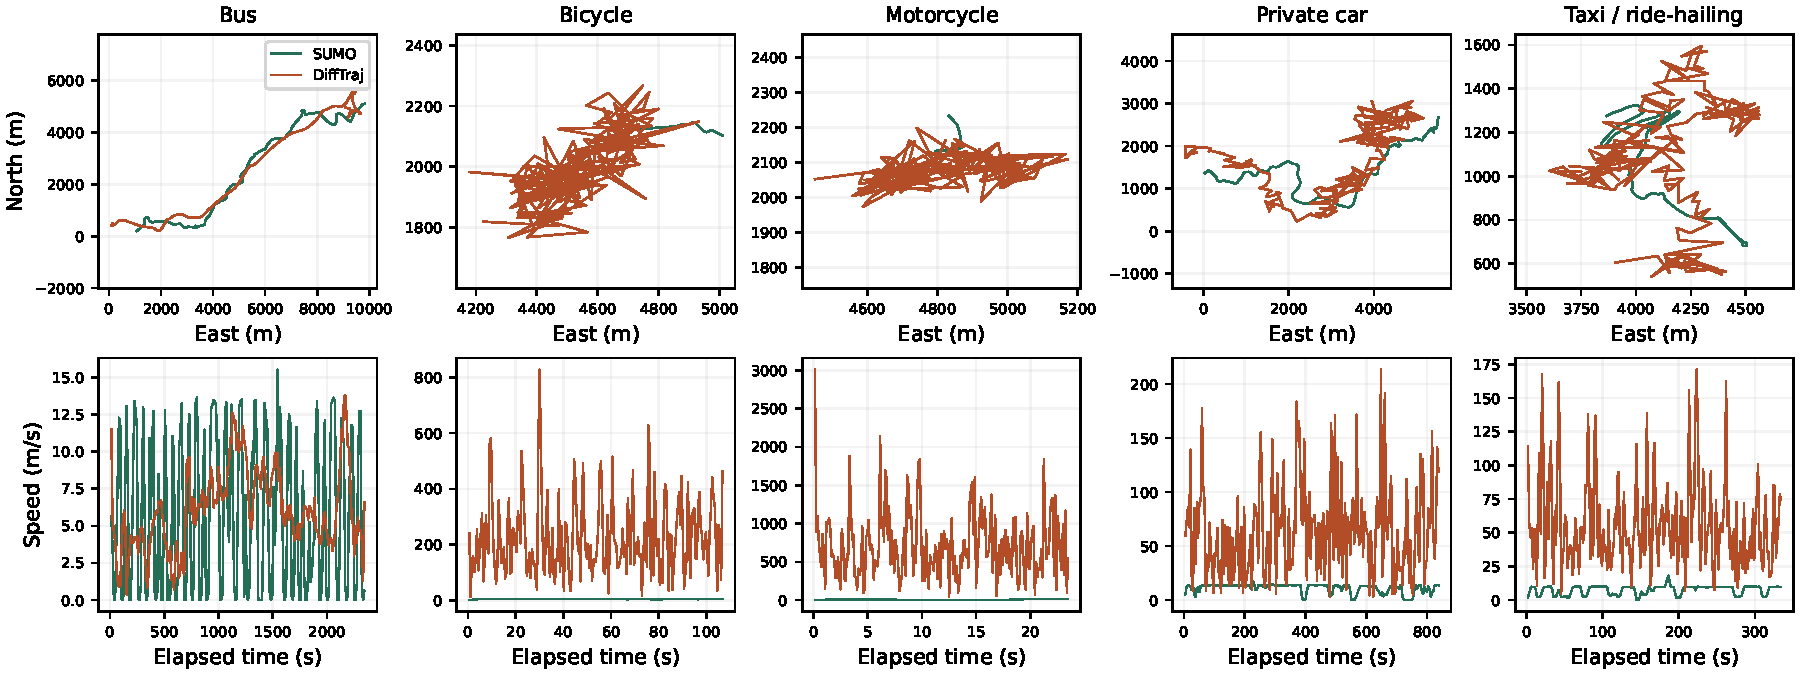
\includegraphics[width=\linewidth]{baseline-examples.pdf}
\caption{The first evaluated request of each class, showing observed and generated positions (top) and interval speeds (bottom). Each column uses its own physical axes. The same coordinate baseline is used for all five cases after 8,000 updates.}\end{figure}
\begin{thebibliography}{5}
\bibitem{difftraj} Y. Zhu et al. DiffTraj: Generating GPS Trajectory with Diffusion Probabilistic Model. NeurIPS, 2023.
\bibitem{vae} D. P. Kingma and M. Welling. Auto-Encoding Variational Bayes. ICLR, 2014.
\bibitem{gan} I. Goodfellow et al. Generative Adversarial Nets. NeurIPS, 2014.
\bibitem{ddpm} J. Ho, A. Jain and P. Abbeel. Denoising Diffusion Probabilistic Models. NeurIPS, 2020.
\bibitem{ddim} J. Song, C. Meng and S. Ermon. Denoising Diffusion Implicit Models. ICLR, 2021.
\end{thebibliography}
\end{document}
